\chapter[Le programme]{Le programme / Interaction avec la scène}
Commençons par une notation pour qualifier les mouvements des cubes. Nous tirons cette notation des Rubik's cubes - c'est ainsi qu'on écrit les algorithmes de résolution du cube. Vous allez comprendre.
\begin{center}
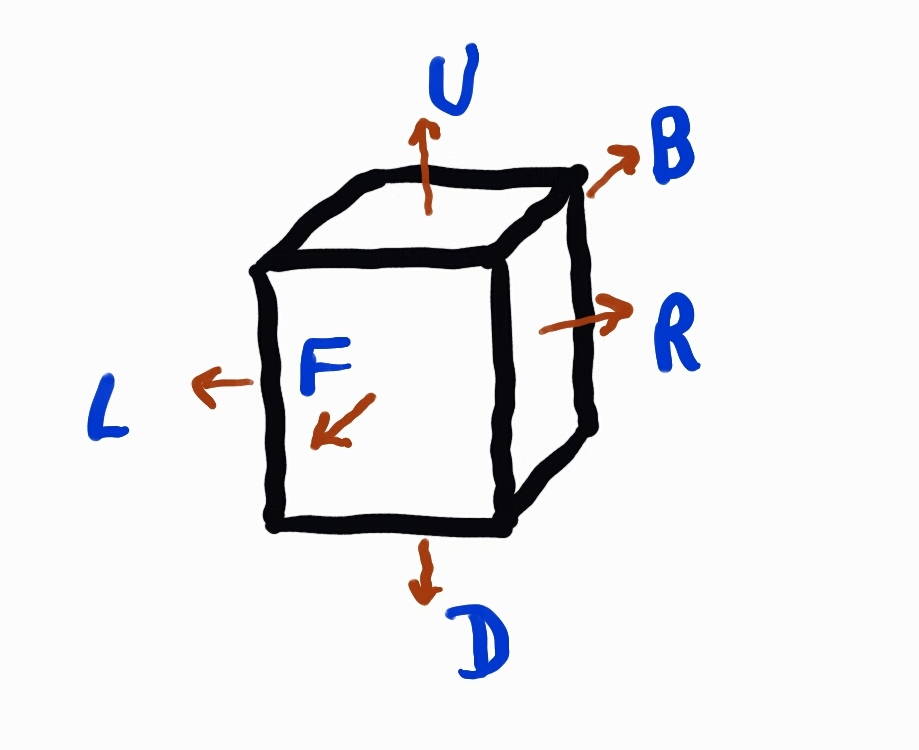
\includegraphics[width=200pt]{Rubik1.jpg}
\end{center}
(Ne vous inquiétez pas... C'est le fond de l'image qui n'est pas blanc, mais bleuté)
\\\\
La notation est la suivante : U pour UP, D pour DOWN, F pour FRONT, B pour BACK, L pour LEFT et R pour RIGHT. Simple, non ? Il suffit de considérer que vous voyez, d'une certaine manière, le cube de face. C'est également ce qui va poser notre choix de caméra pour la scène finale.
\\\\
Du coup, comment décrire les mouvements du cube ? Eh bien, le mouvement "F" indiquera que, si on se place devant la face F, on fait tourner le cube de 90$^{\circ}$ dans le sens horaire. "B" décrira le mouvement inverse (si on se place devant la face B, et qu'on la fait tourner sans le sens horaire, cela revient à faire tourner le cube dans le sens antihoraire si nous sommes face à F). Voici un schéma récapitulatif :
\begin{center}
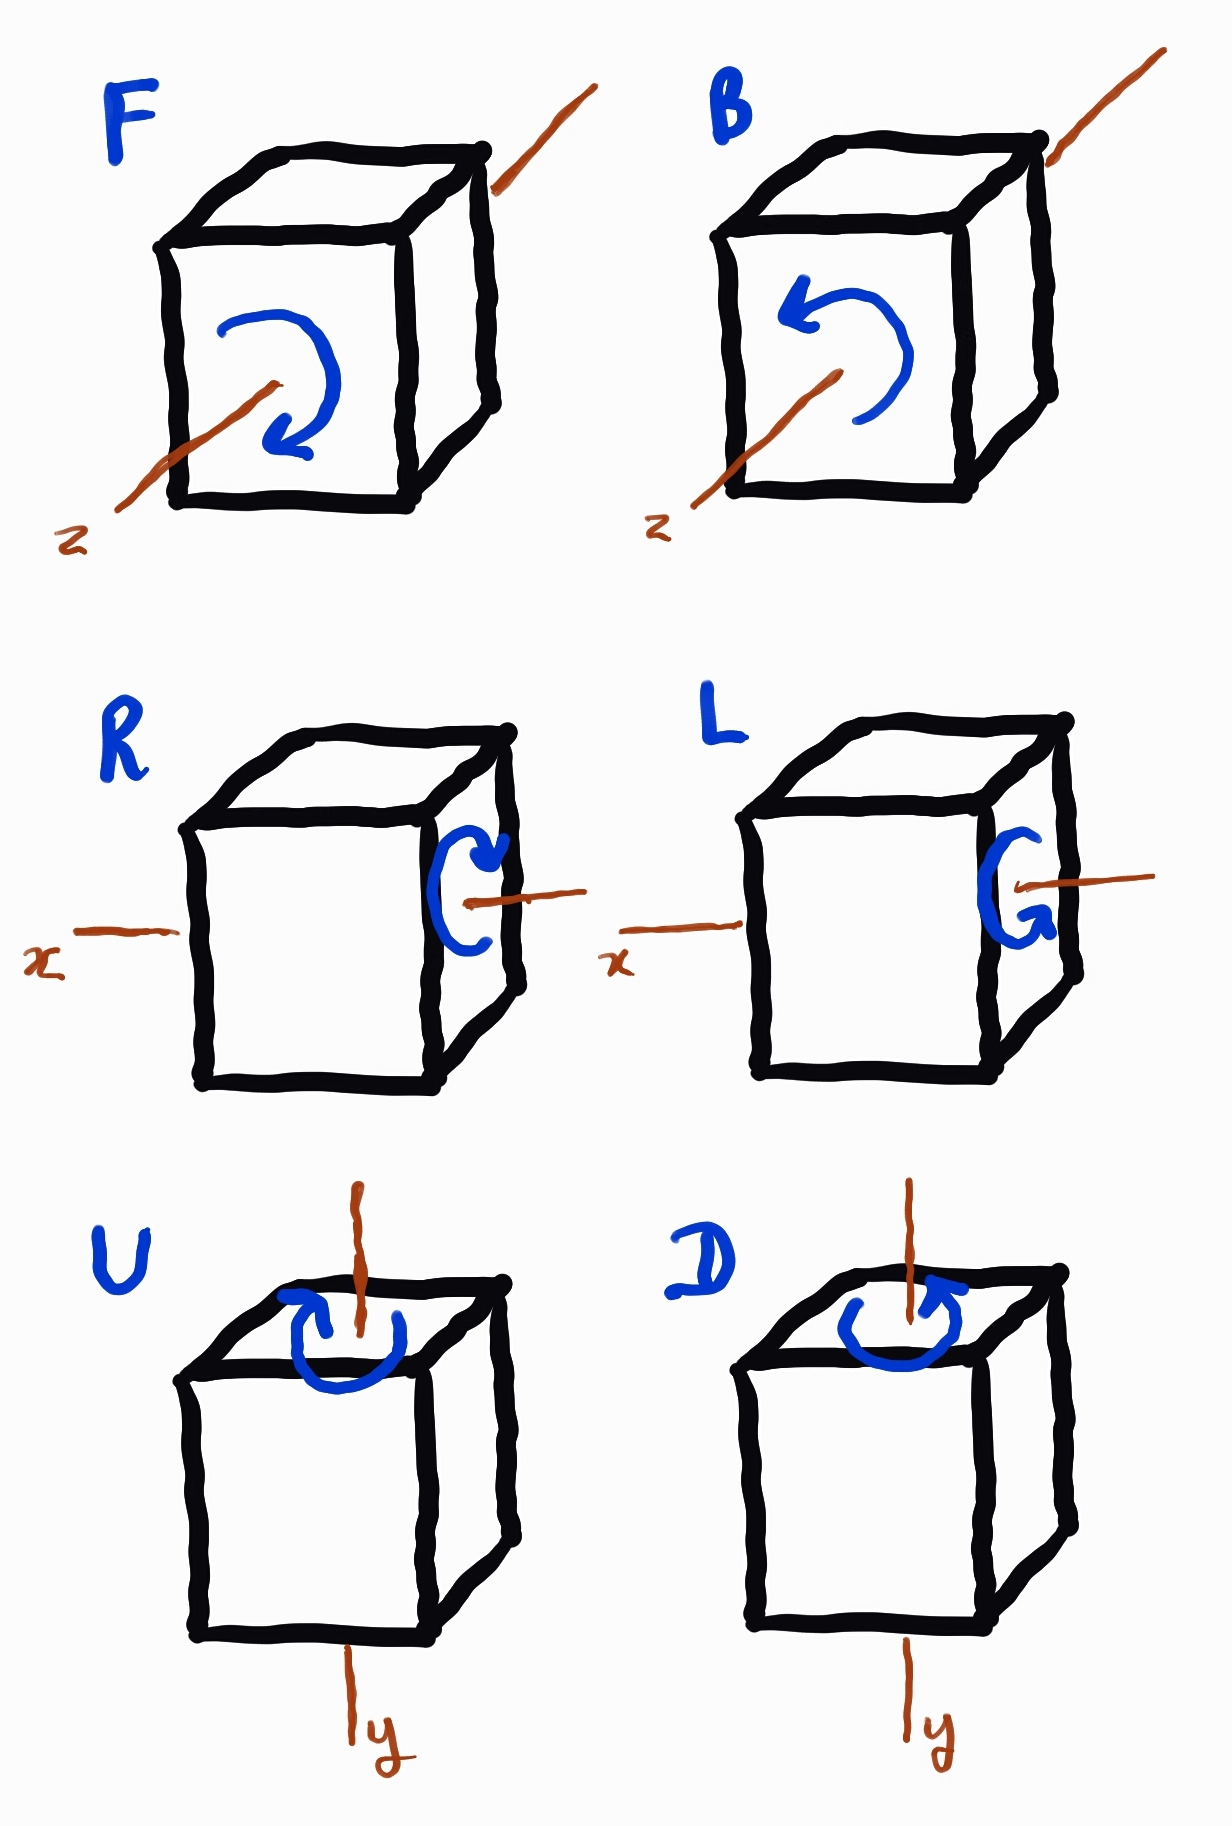
\includegraphics[width=250pt]{Rubik2.jpg}
\end{center}
C'est avec cette notation qu'on décrira les interactions que l'utilisateur aura avec la scène. Évidemment, il s'agit des mouvements par rapport au repère de l'espace, et non pas de la caméra. Si vous vous placez derrière les cubes, tout sera inversé !
\\\\
\begin{tabular}{| c | c || c | c |}
	\hline
	Touche & Caméra & Touche & Cube\\
	\hline \hline
	Z & Avancer & O & Right \\ \hline
	Q & Gauche & K & Up\\ \hline
	S & Reculer & L & Left\\ \hline
	D & Droite & M & Down\\ \hline
	&& I & Back\\ \hline
	&& P & Front\\ \hline
\end{tabular}